%Compilar: pdflatex -synctex=1 -interaction=nonstopmode --shell-escape apuntesed.tex 
\documentclass[10pt,a4paper,spanish]{article}

\usepackage[spanish]{babel}
\usepackage[utf8]{inputenc}
\usepackage{amsmath, amsthm}
\usepackage{amsfonts, amssymb, latexsym}
\usepackage{enumerate}
\usepackage[official]{eurosym}
\usepackage{graphicx}
\usepackage{graphics}
\usepackage[usenames, dvipsnames]{color}
\usepackage{colortbl}
\usepackage{fancyhdr}
\usepackage{fancybox}
\usepackage{pseudocode}
\usepackage[all]{xy}
%\usepackage{minted}
%\usepackage{tikz}
\usepackage{pgfplots}
\usepackage{multirow}
\usepackage{float}
\usepackage{subfigure}
\pgfplotsset{compat=1.5}

% a4large.sty -- fill an A4 (210mm x 297mm) page
% Note: 1 inch = 25.4 mm = 72.27 pt
%       1 pt = 3.5 mm (approx)

% vertical page layout -- one inch margin top and bottom
\topmargin      0 mm    % top margin less 1 inch
\headheight     0 mm    % height of box containing the head
\headsep        10 mm    % space between the head and the body of the page
\textheight     250 mm
\footskip       14 mm    % distance from bottom of body to bottom of foot

\definecolor{denim}{rgb}{0.08, 0.38, 0.74}

\usepackage[bookmarks=true,
            bookmarksnumbered=false, % true means bookmarks in
                                     % left window are numbered
            bookmarksopen=false,     % true means only level 1
                                     % are displayed.
            colorlinks=true,
            linkcolor=webblue]{hyperref}
\definecolor{webgreen}{rgb}{0, 0.5, 0} % less intense green
\definecolor{webblue}{rgb}{0, 0, 0.5}  % less intense blue
\definecolor{webred}{rgb}{0.5, 0, 0}   % less intense red

\newcommand{\HRule}{\rule{\linewidth}{0.5mm}} % regla horizontal para  el titulo

\usepackage[familydefault,light]{Chivo} %% Option 'familydefault' only if the base font of the document is to be sans serif
\usepackage[T1]{fontenc}

\pagestyle{fancy}
%con esto nos aseguramos de que las cabeceras de capítulo y de sección vayan en minúsculas

% \renewcommand{\chaptermark}[1]{%
%       \markboth{#1}{}}
\renewcommand{\sectionmark}[1]{%
      \markright{\thesection\ #1}}
\fancyhf{} %borra cabecera y pie actuales
\fancyhead[LE,RO]{\textcolor{denim}{\bfseries\thepage}}
\fancyhead[LO]{\bfseries\rightmark}
\renewcommand{\headrulewidth}{0.5pt}
\renewcommand{\footrulewidth}{0pt}
\addtolength{\headheight}{0.5pt} %espacio para la raya
\fancypagestyle{plain}{%
      \fancyhead{} %elimina cabeceras en páginas "plain"
      \renewcommand{\headrulewidth}{0pt} %así como la raya
}

%%%%% Para cambiar el tipo de letra en el título de la sección %%%%%%%%%%%
\usepackage{sectsty}
% \chapterfont{\fontfamily{pag}\selectfont} %% for chapter if you want
\sectionfont{\fontfamily{pag}\selectfont}
\subsectionfont{\fontfamily{pag}\selectfont}
\subsubsectionfont{\fontfamily{pag}\selectfont}


%Definimos autor y título
\title{\bf \textcolor{denim}{App para controlar a Zowi}}
\author{Marta Gómez Macías y Braulio Vargas López}


\setlength{\parindent}{0pt}
\setlength{\parskip}{1ex plus 0.5ex minus 0.2ex}

\begin{document}
\maketitle

\tableofcontents

\section{\textcolor{denim}La app}
Hemos hecho una app para controlar a \textit{\textcolor{denim}{Zowi}} mediante gestos y voz. Para ello, hemos partido de una aplicación simple que controlaba a Zowi con botones y que está disponible en \href{https://github.com/jalucenyo/ZowiApp3D}{github}.

Tiene dos vistas principales: la vista para controlar a Zowi mediante gestos y botones (\hyperref[gestos]{Figura \thesection .\ref*{gestos}}) y la vista para controlar a \textit{\textcolor{denim}{Zowi}} mediante voz (\hyperref[voz]{Figura \thesection .\ref*{voz}}). La primera ha sido realizada para la práctica 3 y la última, para la práctica 4.

\begin{figure}[!h]
    \centering
    \mbox{
        \subfigure[Vista para controlar a Zowi mediante gestos y botones]{
            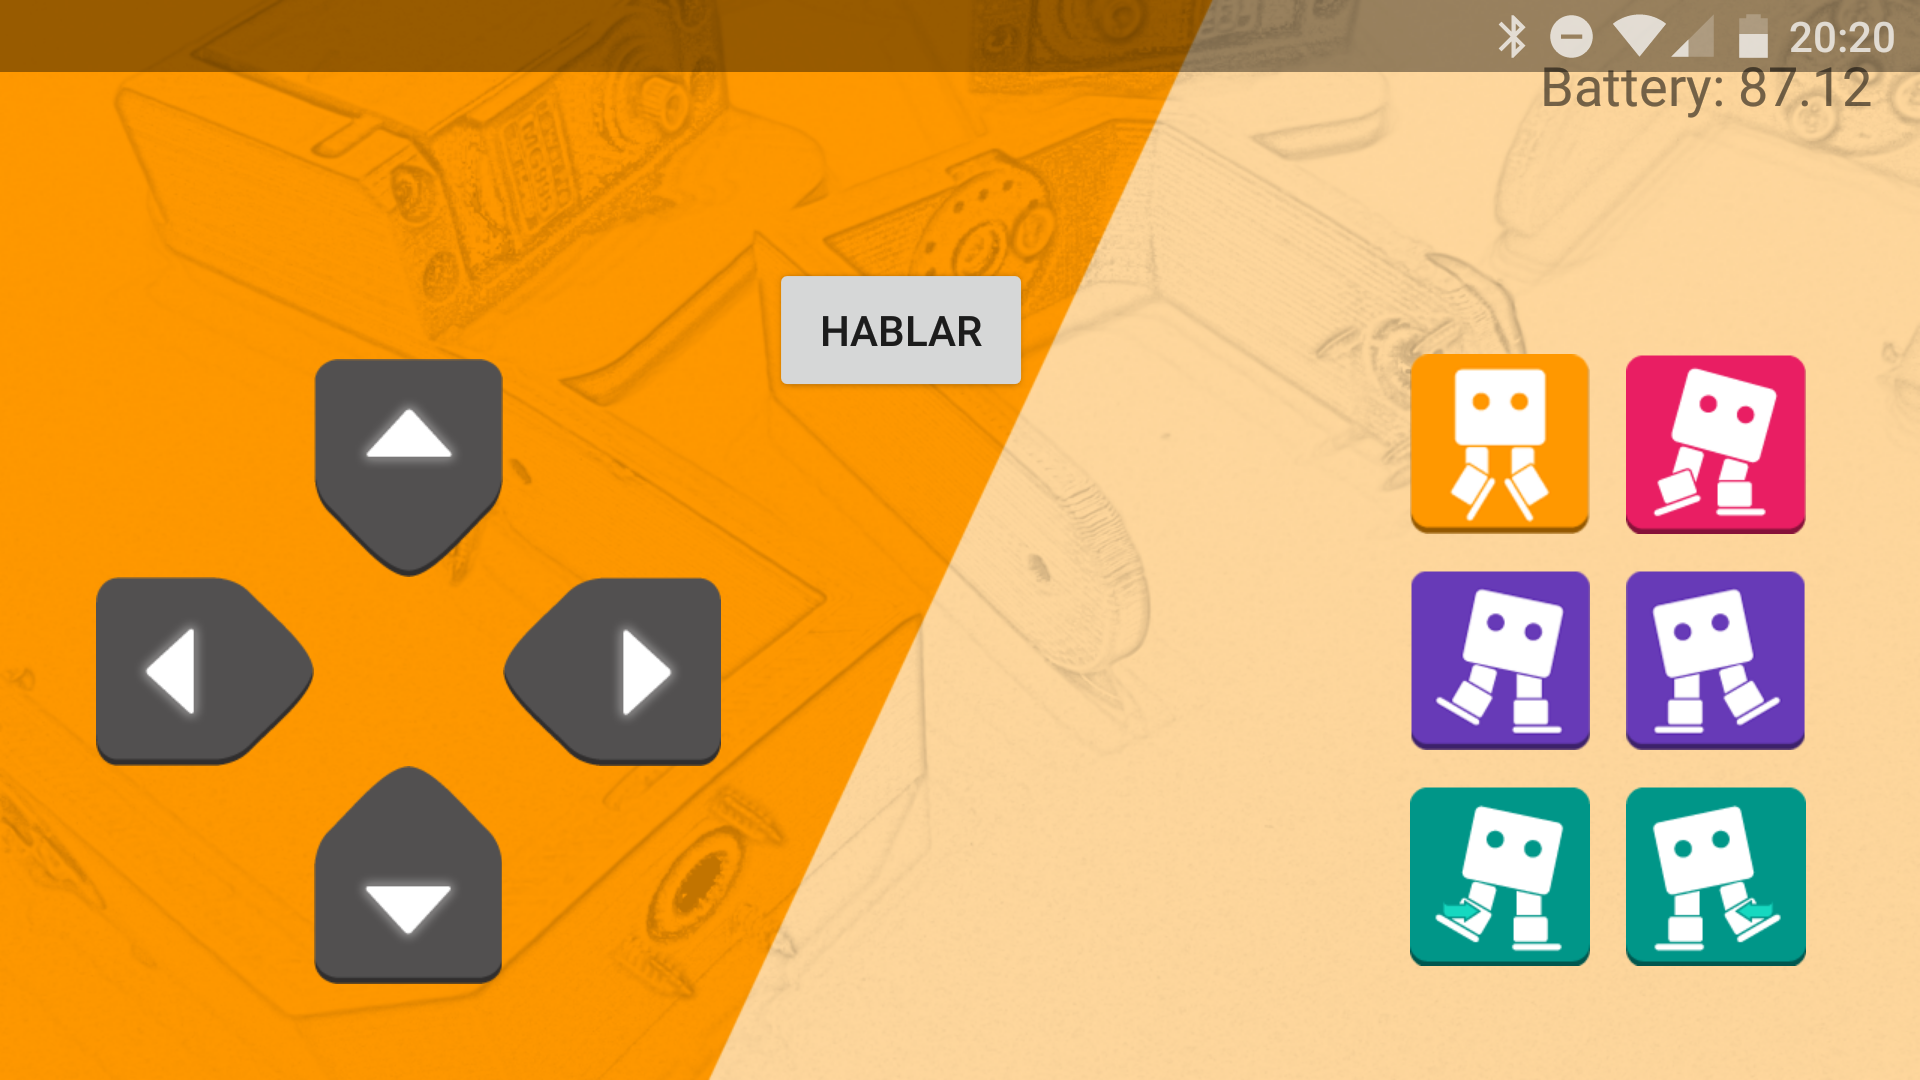
\includegraphics[width=0.5\textwidth]{../screenshots/gestos}
            \label{gestos}
        }
        \subfigure[Vista para controlar a Zowi mediante voz]{
            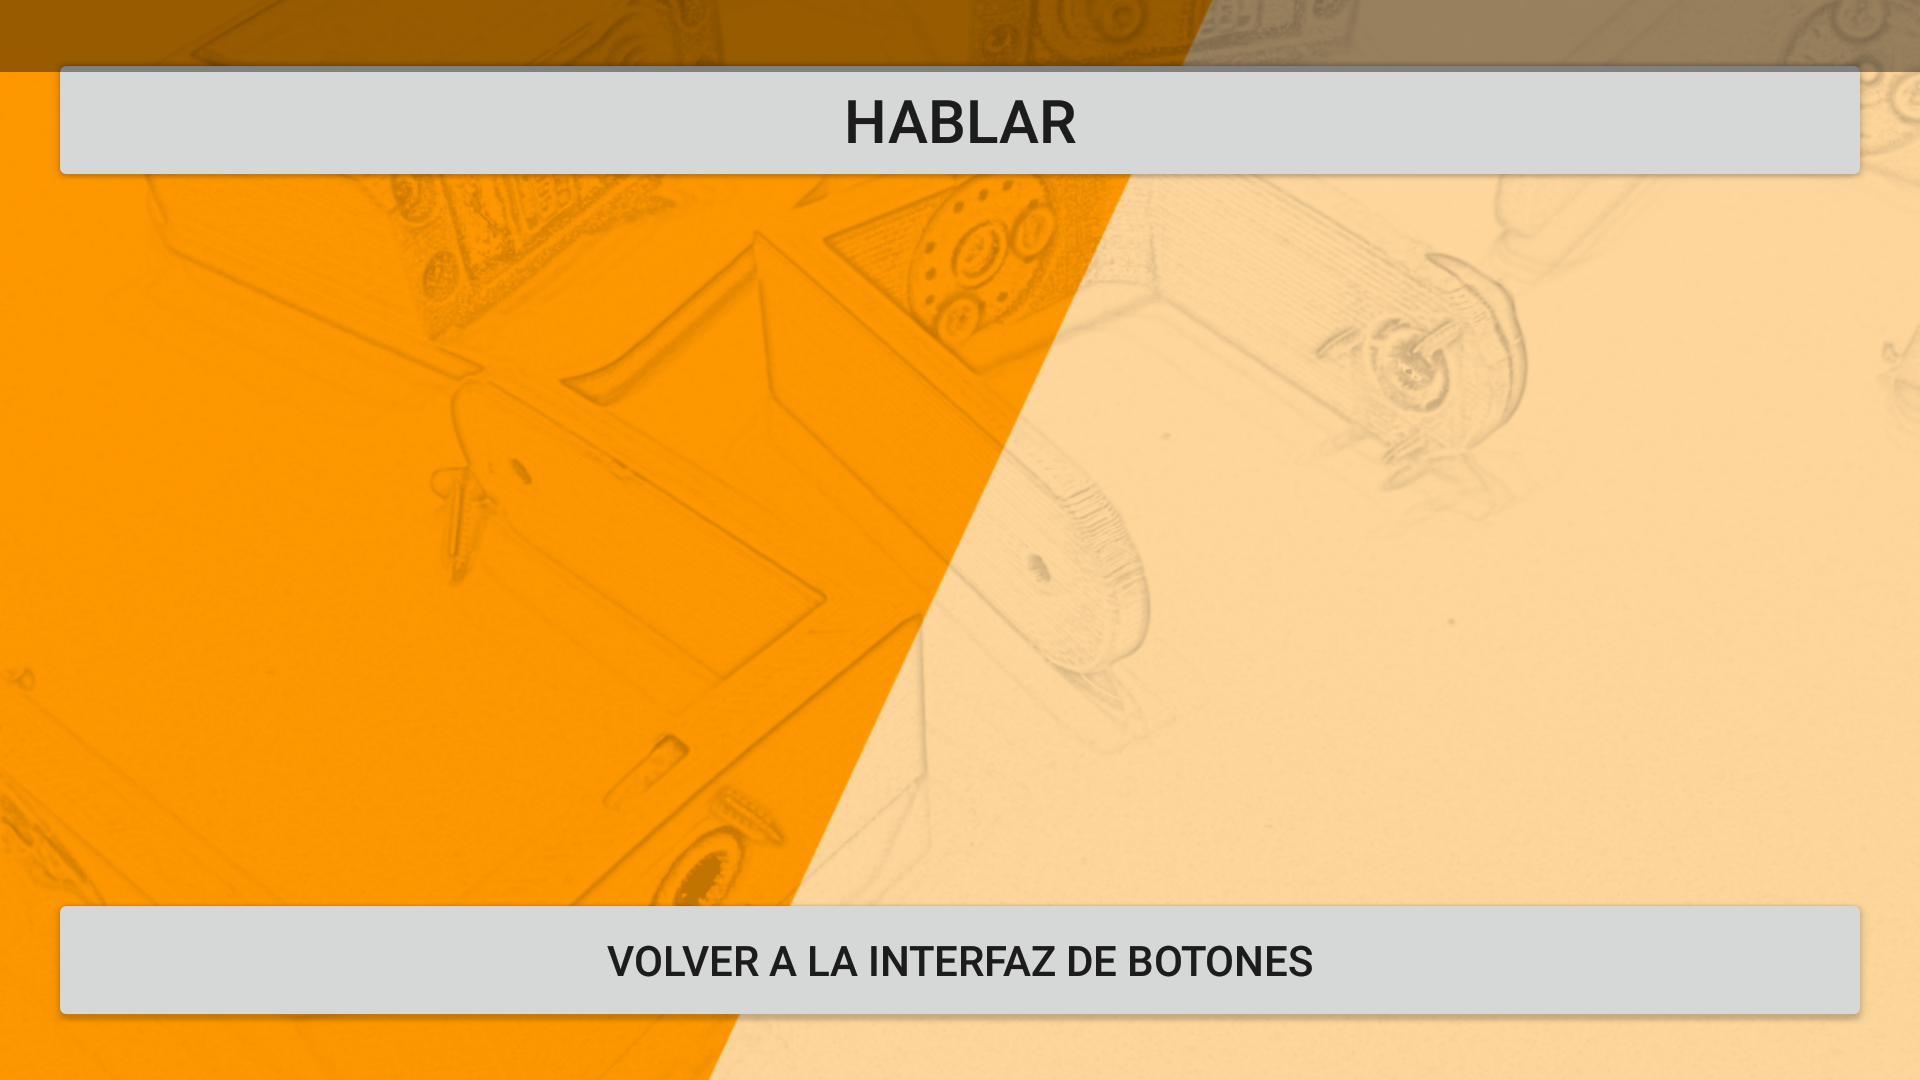
\includegraphics[width=0.5\textwidth]{../screenshots/voz}
            \label{voz}
        }
    }
    \caption{Vistas de la app}
    \label{vistas}
\end{figure}

La app permite hacer que Zowi se mueva y haga distintos pasos de ``baile'' como el \textit{\textcolor{denim}{moonwalk}}, el \textit{\textcolor{denim}{crusaito}} o el \textit{\textcolor{denim}{swing}}.

\section{\textcolor{denim}Interfaz por gestos y botones}
Esta interfaz tiene botones para que \textit{\textcolor{denim}{Zowi}} pueda tanto moverse como bailar, estos botones ya estaban en la app que utilizamos como base. Lo que hemos añadido nosotros han sido gestos para poder controlar la dirección en la que se mueve Zowi usando tanto el \textit{\textcolor{denim}{sensor de rotación}} como el \textit{\textcolor{denim}{acelerómetro}}.

En la \hyperref[axis]{Figura \ref*{axis}} vemos el sistema de coordenadas relativo a un dispositivo que usa Android.

\begin{figure}[!h]
    \centering
    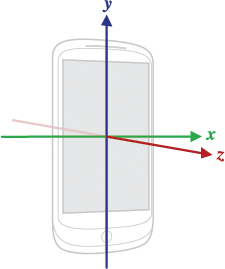
\includegraphics[width=0.2\textwidth]{axis_device}
    \caption{Sistema de coordenadas (relativo a un dispositivo) usado por la Sensor API de Android}
    \label{axis}
\end{figure}

\section{\textcolor{denim}Interfaz por voz}
Esta interfaz tiene sólo dos botones: uno que la app empiece a escuchar al usuario y otro para volver a la interfaz anterior. Esta vista ha sido diseñada a partir de la aplicación de ejemplo facilitada por la profesora \href{https://github.com/zoraidacallejas}{Zoraida Callejas}.

Cuando la app empieza a escuchar al usuario, se llama a la \texttt{\textcolor{denim}{SpeechRecognizer}} de Android. A partir de la frase que se haya reconocido, se busca alguno de los siguientes términos:

\begin{enumerate}[\qquad\ \color{denim}{$\bullet$}]
    \item Jackson
    \item Moonwalk, aunque esta palabra no es reconocida correctamente por lo que no es recomendable usarla.
    \item Swing
    \item Crusaito
    \item Saltar (o salto)
    \item Parar
    \item Ayuda (o podemos decirle a la app que estamos perdidos)
\end{enumerate}

Además, algunas de estas acciones requieren también que le indiquemos la dirección (izquierda o derecha). Si indicamos en la misma frase ambas direcciones, la app nos dará un error diciendo que Zowi sólo puede moverse en una dirección.

\end{document}
